\documentclass[dissertation.tex]{subfiles}
\begin{document}

\chapter{Signatures of Survival Processes in Pancreatic Cancer}
\label{chap:signatures}

\mpfatal{TODO: put the thesis somewhere: That specific molecular processes control survival of resectable PC, and that these processes can be identified and detected using GEX data.}

\section{Introduction}

\paragraph{Summary}Very little is known regarding the biological processes that control the survival of patients with \gls{PDAC}, the most common and aggressive form of pancreas cancer.  As discussed in \cref{chap:nomogram}, the wide range of relative patient survival times that is observed in practice is not well explained by extrinsic factors such as age at diagnosis, and perhaps instead reflects differences in the biological processes operating within each tumour.  Recent molecular profiling work has identified possible molecular subtypes within the previously homogenous group of \gls{PDAC}, but these subtypes have not achieved the maturity or clinical application of those in breast cancer, and their discovery and validation has been hampered by ad-hoc methodology, and the lack of large, well-curated cohorts of \gls{PDAC} samples.  The recently-compiled \gls{APGI} cohort contains the largest group of clinically annotated \gls{PDAC} samples, with accompanying \gls{GEX} and high-quality follow-up data, in the world.  It presents a unique opportunity to apply modern techniques for prognostic signature identification to the discovery of biological processes that drive the clinical course of pancreas cancer.  These signatures may find application as prognostic tools in their own right, but more importantly can supply much-needed information on the fundamental biology of the one common cancer that has, to date, been almost entirely refractory to all the tools of modern molecular medicine.

\vspace{1cm}

Despite extensive research, \gls{PDAC} remains a poorly-understood disease.  Recent genomic profiling has revealed the genetic alterations that accompany the disease \cite{Biankin2012}, and a huge number of prognostic factors are known \cite{Harsha2009}, but these findings have shed little light on the fundamental disease processes at work in individual tumours.  This is a consequence of genetic and biomarker data being poorly-suited for understanding the biological state of a cell: although genetic alterations are central to the etiology of cancer, they give incomplete information on the pathways and systems actually active in a given tumour, and biomarkers supply non-causal readouts of cell state that are difficult to trace back to underlying biological processes.

Sitting between the regulatory function of transcription control, and the effector function of protein expression, \gls{GEX} data integrate information from all aspects of cell condition, including genetic alterations, signalling pathway activity, and metabolic status.  As such, it is unsurprising that \gls{GEX} data are superior indicators of cell state, better than all other high-throughput measurement methods, such as protein expression or genetic alterations \cite{Ray2014}.  However, the involvement of \gls{GEX} with so many biological inputs is also a weakness: typical differential expression studies will identify many hundreds of transcripts that vary between disease states, and the deconvolution of this complex set of hundreds of effects back to a small number of causative molecular processes remains challenging.

Historically, disease \gls{GEX} profiling studies have largely refrained from attempting to infer the state of a few molecular processes from the many hundreds of differentially-expressed genes identified; notable early exceptions are for example \mpfatal{PCA, ICA cites}.  A number of factors are likely to have contributed to this reluctance: deconvolution methods are numerically sensitive and require very large sets of high-quality measurements, early techniques were poorly-suited to the particular requirements of the \gls{GEX} deconvolution problem, and the signature databases that assist the assignation of a biological annotation to the output from a deconvolution calculation (for example, the \acrshort{MSigDB} \cite{Subramanian2005}) have only recently reached maturity.

In addition to the general technical challenges of \gls{GEX} deconvolution, issues particular to pancreas cancer significantly complicate attempts to identify molecular processes at work within the tumours.  Pancreas cancer is challenging to sample, and mRNA in the tissue degrades rapidly once extracted, complicating sample collection.  Additionally, a feature of \gls{PDAC} is the presence of a dense desmoplastic stromal reaction throughout the tumour, that is formed by genetically normal patient stroma cells \cite{Mahadevan2007}.  The fraction of tumour cells that are actually cancerous varies by more than 10-fold between tumours \cite{Biankin2012}, meaning that without careful correction, gene expression profiles are dominated by stromal cell fraction signals, and not true differential expression within a cell type.  Microdissection has been used to separate cancer cells from surrounding stroma in order to simplify analysis \cite{Collisson2011}, but current thought in the field is that the stroma in \gls{PDAC} is an essential and enabling, if not in itself neoplastic, component of the tumour \cite{Mahadevan2007}, and that the examination of cancer cell expression in isolation ignores the likely important interplay between the two major synergistic components of a tumour: transformed epithelial cells, and genetically normal stroma.

Due to these challenges to \gls{GEX} deconvolution of \gls{PDAC}, to date only one study (by Collisson et al) has reported a breakdown of \gls{PDAC} \gls{GEX} into a small number of biological modules \cite{Collisson2011}.  This study examined microdissected cancer cells only, and found that the transformed epithelial cells of \gls{PDAC} could be placed into three major categories, based on their patterns of gene expression.  Tumours from these three categories followed distinct clinical courses, and cell lines exhibited category-specific sensitivity to therapeutic drugs.  As the first report to identify potential clinically relevant molecular subtypes within \gls{PDAC}, the Collisson study was a significant advance in the understanding of the molecular processes at play within what was previously considered a homogeneous disease.  However, it also possesses shortcomings that limit its clinical utility.

Two main issues complicate the interpretation of the Collisson classes: microdissected cancer cells were used, and therefore stromal effects would be severely attenuated; and the deconvolution technique employed was tuned to achieve sample clustering, rather than \gls{GEX} deconvolution.  Consequently, although the Collisson classes could be a fundamental advance in the understanding of \gls{PDAC}, they necessarily do not consider the full context of the disease, and potentially have artifically identified subgroups when in reality a smooth continuum of disease types may exist.  Additionally, although the Collisson tumour subgroups were observed to follow different clinical courses, they were not explicitly generated for this purpose. \mpfatal{Tidy up this last sentence}

A substantial gap remains in our molecular understanding of \gls{PDAC}: little is known about the core molecular processes at work within both the cancer and stroma of different tumours, and almost nothing on those processes that may control patient survival following diagnosis.  Such a gap in knowledge is not merely of academic interest: a better understanding of the processes affecting patient survival can lead directly to improved methods for staging, may stratify patients for customised therapies, and even suggest targets for therapeutics capable of transforming a poor-prognosis cancer into a good-prognosis one.  The primary obstacle for the identification of these survival-associated processes in \gls{PDAC} is one of data: a large, high-quality dataset of \gls{GEX} measurements and associated well-curated \glspl{CPV} is needed.  The \gls{APGI} cohort addresses this data problem for the identification of fundamental survival processes in \gls{PDAC}.  As the largest cohort of \gls{PDAC} samples, with accompanying \gls{GEX} and curated \glspl{CPV}, in the world, it can provide the data quality and cohort size required by modern \gls{GEX} deconvolution techniques.

In this chapter I describe the application of \gls{NMF} for the \gls{GEX} deconvolution of genes associated with outcome.  The metagenes thus identified represent orthogonal coordinately-expressed sets of genes which I then map to biological annotations, identifying the fundamental processes that may be involved in controlling the clinical course of a patient's pancreas cancer.  The results of this work are directly applicable as signatures of survival time following diagnosis of \gls{PDAC}, identify discrete biological processes that appear to determine outcome with pancreas cancer, and highlight fertile future avenues for research into this poorly-understood disease.


\section{Results}

Survival-associated metagenes were identified by selecting the set of genes which had \gls{GEX} associated with outcome in the \gls{APGI} cohort, and then performing \gls{NMF} factorization to deconvolve the full matrix of gene expression signals into a small set of metagenes.  Metagenes were then tested for association with clinical course and other \glspl{CPV}, as well as known general prognostic signatures, and their prognostic ability was validated by 10-fold cross-validation and testing in separate cohorts.  Those metagenes that were found to be prognostic were then correlated with biological process signatures to associate the metagenes with biological processes.

\subsection{Cohort characteristics and subsetting}
The same homogeneous \gls{PDAC} subset of the \gls{APGI} cohort that was used in the work of \cref{chap:nomogram} was employed for this analysis; see \cref{subsec:nomo-results-cohort} on page~\pageref{subsec:nomo-results-cohort} for case selection criteria and cohort characteristics.

\subsection{Three metagenes predict survival with resectable pancreatic cancer in multiple cohorts}
\paragraph{Probe selection}
In order to focus the \gls{GEX} deconvolution method on finding outcome-associated metagenes, it was necessary to filter the full set of gene expression data to only contain those genes that were likely to be associated with patient survival.

A \gls{CPSS} wrapper around the core \gls{SIS}-\gls{FAST} variable selection method \cite{Gorst-Rasmussen2013} identified 361 genes (of 13,000 considered) that were associated with time from diagnosis to disease-specific death in the \gls{APGI} cohort.  50 variable selection runs on permuted data gave a median number of selected genes of 87.5, resulting in an estimated \gls{FDR} for the selection procedure of approximately 25\%.  This relatively high \gls{FDR} was a consequence of the lenient selection parameters used, in an attempt to ensure that even genes for which expression was only weakly prognostic, were included.

\paragraph{Factorization}
The expression of the 361 survival-associated genes across 228 patients was decomposed into metagenes by the \gls{SNMFL} \gls{NMF} algorithm.  The number of metagenes (factorization rank) was automatically estimated to be 6, being the lowest rank for which the improvement in estimation error achieved by adding the next rank, was less than that observed for permuted data (\cref{fig:sigs-nmf-rank}).

\begin{figure}
\centering
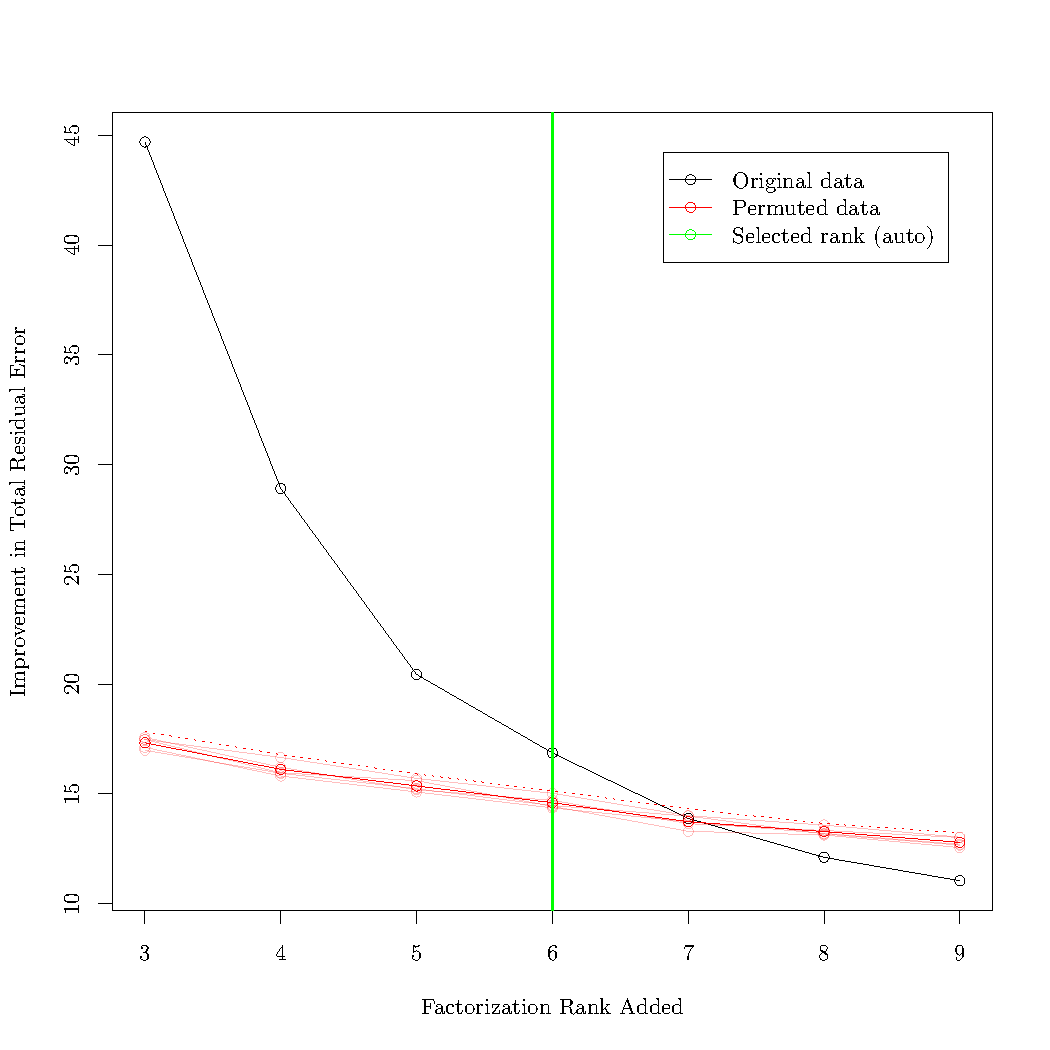
\includegraphics[width=.7\linewidth]{analysis/biosurv/reports/18_SIS_diag_dsd_final/figure/nmf-rank-plots-2}
\caption{Automatic selection of factorization rank.  \acrshort{SNMFL} was performed for varying ranks on either unpermuted data (black line) or data permuted within samples (red lines), and the improvement in total residual approximation error $\|A - W H\|_F$ calculated.  The highest added rank for which the error improvement on unpermuted data exceeded that of permuted data plus two standard deviations (threshold shown by dotted red line) was the final selected rank (green line).\label{fig:sigs-nmf-rank}}
\end{figure}

500 random restarts of rank 6 \gls{SNMFL} were then performed on the survival-associated gene matrix to yield the final factorization.  The resultant clustering consensus matrix was stable (\cref{fig:sigs-nmf-consensus}), and the basis matrix $W$ was reasonably sparse (\cref{fig:sigs-nmf-basis}).  Small row L1 norm of the basis matrix is a desirable condition for this analysis, as it indicates that metagenes are largely distinct transcriptional modules, with little overlap in terms of shared transcripts with high loadings; \gls{SNMFL} was selected against alternative \gls{NMF} algorithms for its design, which favours solutions with small $W$ row L1 norm.  A table of values of the basis matrix $W$ is available as \cref{app:sigs-w-matrix} on \cpagerefrange{app:sigs-w-matrix}{app:sigs-w-matrix-end}.

\begin{figure}
\centering
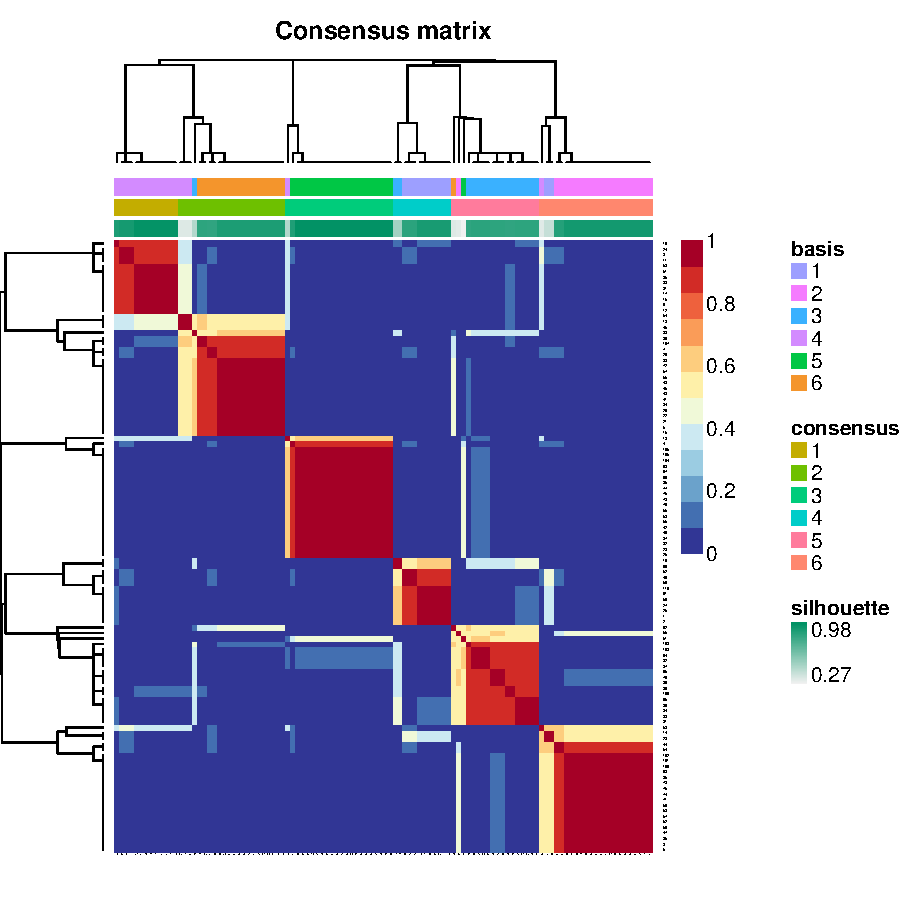
\includegraphics[width=.7\linewidth]{analysis/biosurv/reports/18_SIS_diag_dsd_final/figure/nmf-plots-1}
\caption{Clustering consensus matrix for the final rank-6 clustering.  Colours indicate the stability of gene (in rows) and sample (in columns) clusters across random restarts of the factorization; at rank 6 this factorization was largely stable, with identical clusters assigned in all 500 random restarts to the majority of genes and samples.\label{fig:sigs-nmf-consensus}}
\end{figure}

\begin{figure}
\centering
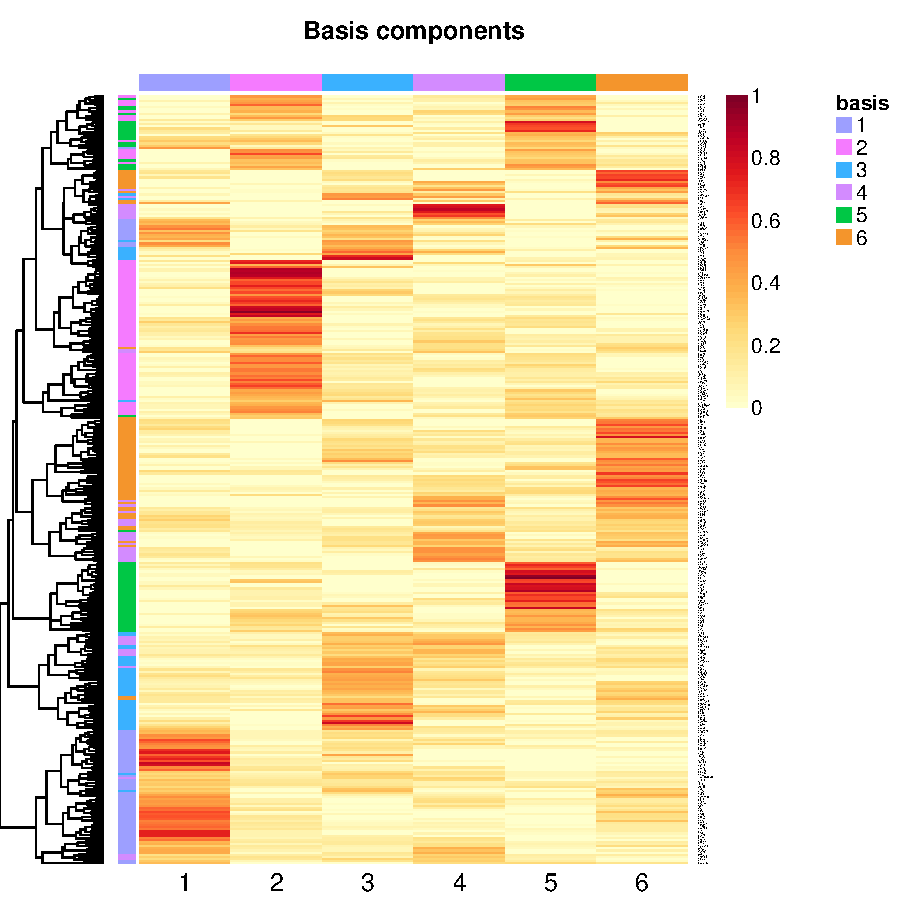
\includegraphics[width=.7\linewidth]{analysis/biosurv/reports/18_SIS_diag_dsd_final/figure/nmf-plots-2}
\caption{Basis matrix $W$ of the final \acrshort{SNMFL} factorization.  Rows represent genes, and columns metagenes, with cell colours proportional to the loading of a given gene on a given metagene.  The loadings are sparse within rows, indicating that the metagenes are modular, each affecting the expression of largely distinct sets of target genes.  A table of values of this basis matrix is available as \cref{app:sigs-w-matrix} on \cpagerefrange{app:sigs-w-matrix}{app:sigs-w-matrix-end}.\label{fig:sigs-nmf-basis}}
\end{figure}

\paragraph{Identifying prognostic metagenes}
The transcription patterns of genes associated with survival in the \gls{APGI} cohort could be decomposed into just six largely distinct metagenes.  Due to the presence of false positives in the 361 screened input genes, some of the metagenes will have no strong association with outcome.  To identify which of the six metagenes were ultimately predictive of patient survival, I performed \gls{LASSO} regression on the \gls{APGI} discovery cohort data, using \gls{NNLS}-estimated coefficients of each of the six metagenes as marginal predictors of outcome.  The \gls{LASSO} regularization parameter $\lambda$ was chosen by 10-fold cross-validation to be the highest value for which the mean test set partial likelihood deviance was within one standard error of the lowest mean value.  This resulted in a final model in which three metagenes, MG1, MG2, and MG5, were selected as prognostic (\cref{fig:sigs-resub-lasso-track}).

\begin{figure}
\centering
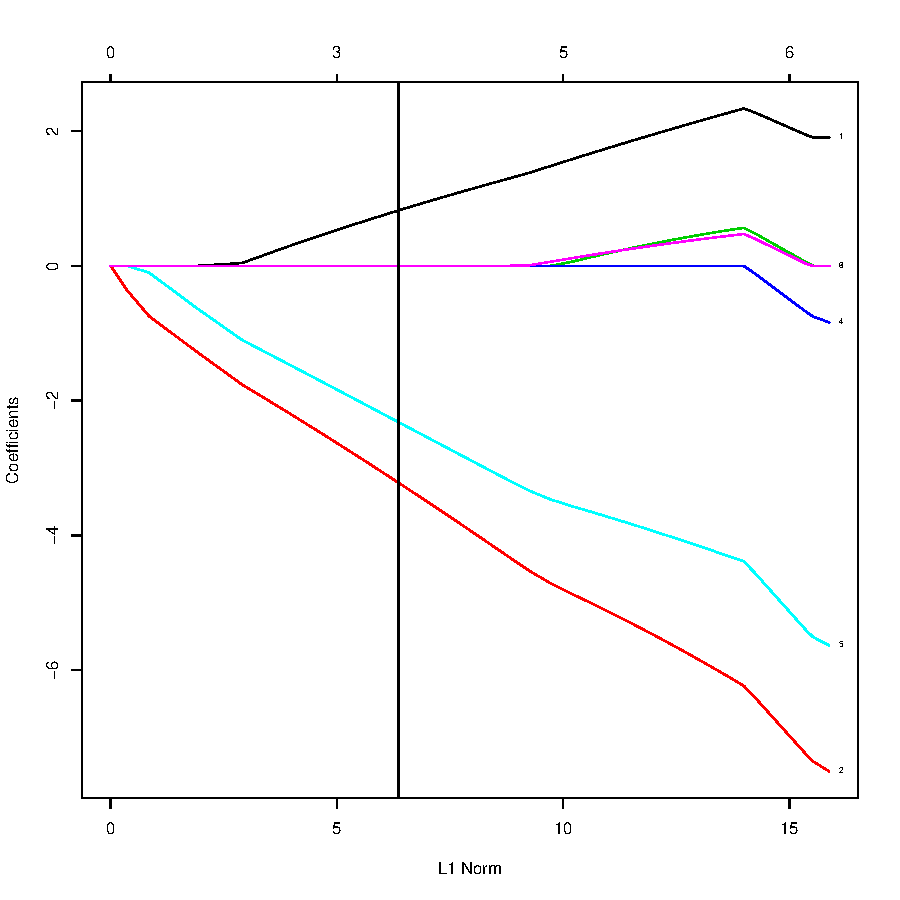
\includegraphics[width=.7\linewidth]{analysis/biosurv/reports/18_SIS_diag_dsd_final/figure/nmf-metagene-glmnet-plots-2}
\caption{Coefficient vs penalty fit trajectories for the \acrshort{LASSO} model predicting disease-specific survival from metagene expression.  Each line represents the model coefficient for a metagene as the model is smoothly varied from a null model (L1 norm = 0), to a full unpenalised Cox fit (L1 norm $\approx$ 16).  The vertical line indicates the optimal value of L1 norm as selected by 10-fold cross-validation; at this point in the trajectory only metagenes MG1, MG2, and MG5 contribute to prognosis estimates.\label{fig:sigs-resub-lasso-track}}
\end{figure}

The final signature developed for predicting time from diagnosis to death for patients \gls{PDAC} therefore consists of three distinct metagenes: the protective MG2 and MG5, and the hazardous MG1.  For external validation of the signature I combined observed coefficients for the three metagenes using their CV-selected \gls{APGI} cohort \gls{LASSO} fit coefficients, as $\text{Risk score} = 0.8238 \times \text{MG1 coefficient} - 3.2195 \times \text{MG2 coefficient} - 2.3208 \times \text{MG5 coefficient}$.  Full metagene scores for the 361 survival-associated genes (the $W$ matrix) are available as \cref{app:sigs-w-matrix} on \cpagerefrange{app:sigs-w-matrix}{app:sigs-w-matrix-end}.

\paragraph{Validation of the three-metagene signature}
To ensure that the process for development of the three-metagene survival signature was reproducible, and that the signature itself was transferable to other cohorts, I performed cross- and external validation of the metagene survival signature.  10-fold cross-validation was performed on the full metagene discovery procedure, from supervised probe selection by \gls{CPSS}-\gls{SIS}-\gls{FAST} to final \gls{LASSO} coefficient estimation, including automatic \gls{NMF} rank estimation.  Cross-validated test set risk scores from the \gls{APGI} discovery cohort were significantly predictive of time from diagnosis to disease-specific death by Cox regression (LRT $P = $\mpfatal{Update with new data}).  The three-metagene survival signature described above also validated against the \gls{PDAC} expression cohort GSE28735 \cite{Zhang2013} (LRT $P = 0.0139$), demonstrating the robustness of the metagene signature to cohort and platform effects.  \mpfatal{Talk about GSE21501 here}

\subsection{Prognostic metagenes define two axes of cell state and survival}
To link metagene expression with potential underlying biology, metagene coefficients on the \gls{APGI} discovery cohort were compared to clinical variates, scores of a general prognostic signature, and scores for signatures from the \gls{MSigDB} \cite{Subramanian2005}.

Correlations between metagene coefficients and \gls{MSigDB} scores revealed a parity in the metagenes: MG1 and MG5, MG2 and MG6, and MG3 and MG4, formed complementary pairs in terms of their correlation with \gls{MSigDB} signatures (\cref{fig:sigs-nmf-corplots}).  This parity reflects mutual exclusivity interactions between metagene coefficients, and suggests that the six metagenes encode only three underlying biological states.  The three prognostic metagenes were therefore combined into two prognostic axes: MG2-MG6, and MG5-MG1.

\begin{figure}
\centering
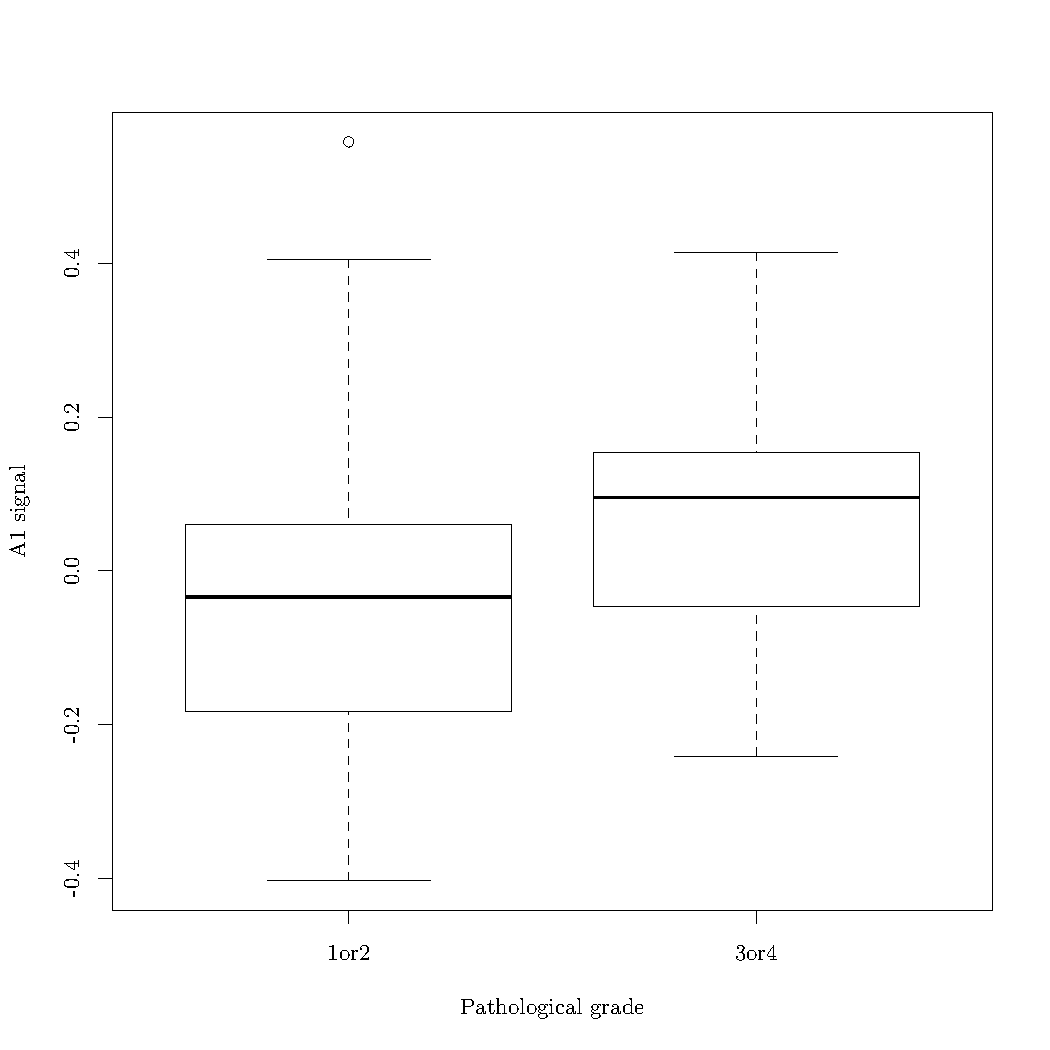
\includegraphics[width=.7\linewidth]{analysis/biosurv/reports/18_SIS_diag_dsd_final/figure/nmf-msigdb-cor-plots-1}
\caption{Correlations between metagenes and \acrshort{MSigDB} signatures.  Metagene coefficients, and \acrshort{GSVA} \acrshort{MSigDB} signature scores, were calculated on the \acrshort{APGI} \acrshort{GEX} data.  Kendall's correlation coefficients were then calculated between the scores of each metagene and signature pair, and are plotted here.  Metagenes MG1 and MG5, MG2 and MG6, and MG3 and MG4, form complementary pairs in terms of their correlation patterns with \acrshort{MSigDB} signatures.\label{fig:sigs-nmf-corplots}}
\end{figure}

\gls{MSigDB} correlations, as well as comparisons to a general survival signature, revealed that the MG5-MG1 axis primarily reflected the proliferative state of cells.  Coefficients of the hazardous MG1 were strongly correlated with scores of the general outcome predictor meta-PCNA (Kendall's $\tau = 0.757$, $n = 110$), a 130 gene signature of cell proliferation \cite{Venet2011} (\cref{fig:sigs-mg1-pcna}).  Supporting this finding, MG1 coefficients were also strongly associated with \gls{GSVA} estimates of the E2F1 response, and of a number of cell-cycle related \gls{MSigDB} sets (\cref{tab:sigs-msigdb-corrs-mg15}).  Coefficients for the protective MG5 were significantly negatively correlated with qPure estimates of cancer cell fraction \cite{Song2012} (\cref{tab:sigs-mg-cpvs}), and positively correlated with the \gls{GSVA} score of genes with promoter regions within $\pm 2\ \text{kb}$ of the STAT5A target motif \texttt{AWTTCYNGGAANY}.  Taken together, these associations suggest that a high MG1 coefficient (equivalently, a low MG5 coefficient) is a marker of aggressive tumours with high proliferative activity, relatively low stromal content, and poor outcome.  Conversely, high a MG5 coefficient (low MG1) indicates a less aggressive tumour with higher stromal content, and possibly increased immune involvement.

\begin{figure}
\centering
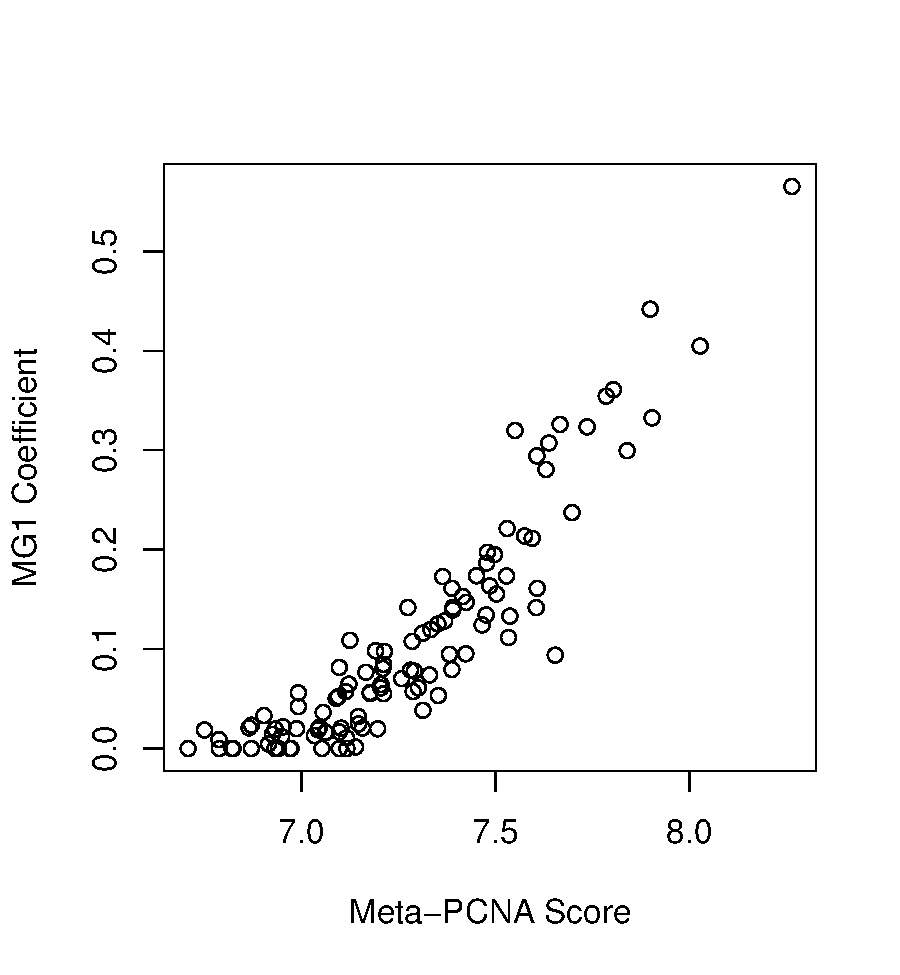
\includegraphics[width=.7\linewidth]{analysis/biosurv/reports/18_SIS_diag_dsd_final/figure/metagene-pairs-7}
\caption{MG1 coefficients are closely associated with meta-PCNA signature score.  MG1 coefficients and meta-PCNA \cite{Venet2011} scores were as evaluated on the \gls{APGI} training set; Kendall's $\tau = 0.757$, $n = 110$.\label{fig:sigs-nmf-corplots}}
\end{figure}

\begin{table}[ht]
\caption{\acrshort{MSigDB} signatures substantially correlated to the MG5-MG1 axis.\label{tab:sigs-msigdb-corrs-mg15}}
\centering
\begin{tabularx}{\textwidth}{ @{} X l l @{} }
  \toprule
   & \multicolumn{2}{c}{Correlation} \\
  MSigDB Signature & MG1 & MG5 \\ 
  \midrule
  c2 REACTOME G\textsubscript{S}$\alpha$ signalling events & -0.36 & 0.55 \\ 
  c5 Phosphoric diester hydrolase activity & -0.35 & 0.52 \\ 
  c3 V\$STAT5A 01 & -0.31 & 0.52 \\ 
  ... & ... & ... \\
%  c5 3 5 CYCLIC NUCLEOTIDE PHOSPHODIESTERASE ACTIVITY, & -0.23 & 0.52 \\ 
%  c5 CYCLIC NUCLEOTIDE PHOSPHODIESTERASE ACTIVITY & & \\
%  c6 SINGH KRAS DEPENDENCY SIGNATURE  & 0.20.& -0.51 \\ 
%  c3 SGCGSSAAA V\$E2F1DP2 01 & 0.51 & -0.21 \\ 
%  c2 REACTOME INTERACTIONS OF VPR WITH HOST CELLULAR PROTEINS & 0.52 & -0.21 \\ 
%  c5 DNA REPLICATION & 0.53 & -0.21 \\ 
%  c2 REACTOME NEP NS2 INTERACTS WITH THE CELLULAR EXPORT MACHINERY & 0.53 & -0.25 \\ 
%  c2 REACTOME TRANSPORT OF RIBONUCLEOPROTEINS INTO THE HOST NUCLEUS, & & \\
%  c2 REACTOME REGULATION OF GLUCOKINASE BY GLUCOKINASE REGULATORY PROTEIN & & \\
%  c2 REACTOME TRANSPORT OF MATURE MRNA DERIVED FROM AN INTRONLESS TRANSCRIPT & 0.52 & -0.27 \\ 
%  c6 AKT UP V1 SIGNED & 0.26 & -0.52 \\ 
%  c2 PID ATM PATHWAY & 0.52 & -0.27 \\ 
%  c2 REACTOME ANTIVIRAL MECHANISM BY IFN STIMULATED GENES & 0.54 & -0.26 \\ 
%  c2 REACTOME METABOLISM OF NON CODING RNA & 0.51 & -0.30 \\ 
%  c3 V\$E2F Q3 01, & 0.52 & -0.30 \\ 
%  c3 V\$E2F1 Q4 01 & & \\
%  c2 REACTOME PROCESSIVE SYNTHESIS ON THE LAGGING STRAND & 0.52 & -0.29 \\ 
%  c3 V\$E2F Q4 01 & 0.54 & -0.29 \\ 
%  c2 REACTOME HIV INFECTION, & 0.54 & -0.29 \\ 
%  c2 REACTOME HOST INTERACTIONS OF HIV FACTORS & & \\
%  c3 V\$E2F Q6 01 & 0.53 & -0.31 \\ 
%  c4 MORF PCNA & 0.51 & -0.33 \\ 
%  c5 DNA POLYMERASE ACTIVITY, & 0.52 & -0.33 \\ 
%  c5 DNA DIRECTED DNA POLYMERASE ACTIVITY & & \\
%  c2 REACTOME REPAIR SYNTHESIS FOR GAP FILLING BY DNA POL IN TC NER & 0.51 & -0.34 \\ 
%  c2 KEGG OOCYTE MEIOSIS & 0.55 & -0.31 \\ 
%  c2 REACTOME HIV LIFE CYCLE, & 0.51 & -0.35 \\ 
%  c2 REACTOME LATE PHASE OF HIV LIFE CYCLE & & \\
%  c6 E2F1 UP V1 SIGNED & 0.53 & -0.34 \\ 
%  c4 GNF2 MSH6 & 0.52 & -0.34 \\ 
%  c2 REACTOME APOPTOSIS & 0.51 & -0.35 \\ 
%  c5 INTERPHASE, & 0.52 & -0.35 \\ 
%  c5 INTERPHASE OF MITOTIC CELL CYCLE & & \\
%  c5 REGULATION OF CELL CYCLE & 0.55 & -0.32 \\ 
%  c5 MICROTUBULE CYTOSKELETON ORGANIZATION AND BIOGENESIS & 0.53 & -0.35 \\ 
%  c2 REACTOME REGULATION OF MRNA STABILITY BY PROTEINS THAT BIND AU RICH ELEMENTS & 0.52 & -0.37 \\ 
%  c2 REACTOME DNA REPAIR & 0.52 & -0.37 \\ 
%  c2 REACTOME ORC1 REMOVAL FROM CHROMATIN, & 0.57 & -0.31 \\ 
%  c2 REACTOME M G1 TRANSITION, & & \\
%  c2 REACTOME ASSEMBLY OF THE PRE REPLICATIVE COMPLEX & & \\
%  c2 REACTOME CHROMOSOME MAINTENANCE, & 0.53 & -0.36 \\ 
%  c2 REACTOME TELOMERE MAINTENANCE & & \\
%  c2 REACTOME LAGGING STRAND SYNTHESIS, & 0.56 & -0.33 \\ 
%  c2 REACTOME EXTENSION OF TELOMERES & & \\
%  c5 RESPONSE TO ENDOGENOUS STIMULUS, & 0.51 & -0.39 \\ 
%  c5 RESPONSE TO DNA DAMAGE STIMULUS & & 
%  c2 REACTOME CYCLIN E ASSOCIATED EVENTS DURING G1 S TRANSITION, & 0.56 & -0.34 \\ 
%  c2 REACTOME REGULATION OF MITOTIC CELL CYCLE, & & \\
%  c2 REACTOME APC C CDH1 MEDIATED DEGRADATION OF CDC20 AND OTHER APC C CDH1 TARGETED PROTEINS IN LATE MITOSIS EARLY G1, & & \\
%  c2 REACTOME APC C CDC20 MEDIATED DEGRADATION OF MITOTIC PROTEINS, & & \\
%  c2 REACTOME SCFSKP2 MEDIATED DEGRADATION OF P27 P21 & & \\
%  c2 REACTOME UNWINDING OF DNA & 0.59 & -0.31 \\ 
%  c5 CHROMOSOMEPERICENTRIC REGION, & 0.53 & -0.38 \\ 
%  c5 KINETOCHORE & & \\
%  c5 CHROMOSOMAL PART, & 0.57 & -0.33 \\ 
%  c5 CHROMOSOME & & \\
%  c5 MITOTIC SISTER CHROMATID SEGREGATION, & 0.52 & -0.39 \\ 
%  c5 SISTER CHROMATID SEGREGATION & & \\
%  c2 PID AURORA B PATHWAY & 0.59 & -0.33 \\ 
%  c4 MORF CCNF & 0.54 & -0.38 \\ 
%  c5 DNA METABOLIC PROCESS & 0.57 & -0.36 \\ 
%  c3 SCGGAAGY V\$ELK1 02 & 0.41 & -0.52 \\ 
%  c4 MORF DNMT1 & 0.51 & -0.42 \\ 
%  c2 REACTOME POL SWITCHING & 0.54 & -0.39 \\ 
%  c4 GNF2 MSH2 & 0.58 & -0.35 \\ 
%  c4 MORF UNG & 0.52 & -0.42 \\ 
%  c2 KEGG DNA REPLICATION, & 0.61 & -0.32 \\ 
%  c2 REACTOME DNA STRAND ELONGATION & & \\
%  c2 PID BARD1PATHWAY & 0.57 & -0.37 \\ 
%  c5 CHROMOSOME SEGREGATION & 0.51 & -0.43 \\ 
%  c2 PID AURORA A PATHWAY & 0.58 & -0.36 \\ 
%  c2 REACTOME G2 M DNA DAMAGE CHECKPOINT & 0.59 & -0.35 \\ 
%  c5 SPINDLE MICROTUBULE & 0.56 & -0.38 \\ 
%  c4 GNF2 PA2G4, & 0.53 & -0.41 \\ 
%  c4 GNF2 RAN & & \\
%  c3 V\$ELK1 02 & 0.45 & -0.50.\\ 
%  c4 GNF2 MCM5 & 0.57 & -0.39 \\ 
%  c2 PID ATR PATHWAY & 0.61 & -0.35 \\ 
%  c4 MORF BUB1 & 0.56 & -0.42 \\ 
%  c5 CELL CYCLE CHECKPOINT GO 0000075 & 0.63 & -0.35 \\ 
%  c2 REACTOME KINESINS & 0.60.& -0.38 \\ 
%  c4 MORF BUB3, & 0.51 & -0.47 \\ 
%  c4 MORF RAD23A & & \\
%  c4 MORF RFC4, & 0.53 & -0.46 \\ 
%  c4 MORF RRM1 & & \\
%  c5 MITOTIC SPINDLE ORGANIZATION AND BIOGENESIS, & 0.62 & -0.37 \\ 
%  c5 SPINDLE ORGANIZATION AND BIOGENESIS & & \\
%  c2 PID FOXM1PATHWAY & 0.61 & -0.38 \\ 
%  c2 REACTOME E2F ENABLED INHIBITION OF PRE REPLICATION COMPLEX FORMATION & 0.57 & -0.43 \\ 
%  c2 REACTOME METABOLISM OF NUCLEOTIDES & 0.46 & -0.54 \\ 
%  c5 MITOTIC CELL CYCLE CHECKPOINT & 0.62 & -0.39 \\ 
%  c4 MORF ESPL1 & 0.60.& -0.41 \\ 
%  c5 CELL CYCLE GO 0007049 & 0.65 & -0.36 \\ 
%  c4 MORF FEN1 & 0.62 & -0.39 \\ 
%  c2 REACTOME E2F MEDIATED REGULATION OF DNA REPLICATION & 0.62 & -0.40 \\ 
%  c2 REACTOME CELL CYCLE CHECKPOINTS, & 0.65 & -0.37 \\ 
%  c2 REACTOME G1 S TRANSITION, & & \\
%  c2 REACTOME SYNTHESIS OF DNA, & & \\
%  c2 REACTOME MITOTIC G1 G1 S PHASES, & & \\
%  c2 REACTOME MITOTIC M M G1 PHASES, & & \\
%  c2 REACTOME DNA REPLICATION, & & \\
%  c2 REACTOME S PHASE
%  c5 SPINDLE POLE & 0.58 & -0.45 \\ 
%  c2 REACTOME G1 S SPECIFIC TRANSCRIPTION & 0.58 & -0.45 \\ 
%  c2 PID PLK1 PATHWAY & 0.57 & -0.46 \\ 
%  c5 ORGANELLE PART, & 0.54 & -0.49 \\ 
%  c5 INTRACELLULAR ORGANELLE PART & & \\
%  c2 REACTOME MITOTIC PROMETAPHASE & 0.64 & -0.40.\\ 
%  c2 REACTOME CYCLIN A B1 ASSOCIATED EVENTS DURING G2 M TRANSITION & 0.61 & -0.43 \\ 
%  c2 REACTOME ACTIVATION OF THE PRE REPLICATIVE COMPLEX, & 0.68 & -0.36 \\ 
%  c2 REACTOME ACTIVATION OF ATR IN RESPONSE TO REPLICATION STRESS, & & \\
%  c2 REACTOME G2 M CHECKPOINTS & & \\
%  c2 KEGG CELL CYCLE & 0.66 & -0.40 \\ 
%  c6 CSR LATE UP V1 SIGNED & 0.56 & -0.50 \\ 
%  c2 KAMMINGA EZH2 TARGETS, & 0.65 & -0.42 \\ 
%  c4 GNF2 FEN1, & & \\
%  c4 GNF2 RRM1, & & \\
%  c4 GNF2 SMC4L1 & & \\
%  c5 SPINDLE & 0.65 & -0.42 \\ 
%  c4 MORF BUB1B & 0.65 & -0.43 \\ 
%  c2 REACTOME CELL CYCLE, & 0.68 & -0.41 \\ 
%  c2 REACTOME CELL CYCLE MITOTIC & & \\
%  c5 CELL CYCLE PROCESS, & 0.68 & -0.45 \\ 
%  c5 MITOTIC CELL CYCLE, & & \\ 
%  c5 CELL CYCLE PHASE & & \\
%  c2 EGUCHI CELL CYCLE RB1 TARGETS, & 0.70.& -0.43 \\ 
%  c2 ROSTY CERVICAL CANCER PROLIFERATION CLUSTER, & & \\
%  c4 GNF2 BUB1, & & \\
%  c4 GNF2 ESPL1, & & \\
%  c4 GNF2 PCNA, & & \\
%  c4 GNF2 RRM2, & & \\
%  c4 GNF2 BUB1B, & & \\
%  c4 GNF2 MCM4
%  c5 REGULATION OF MITOSIS & 0.65 & -0.50 \\ 
%  c4 GNF2 RFC3, & 0.70 & -0.45 \\ 
%  c4 GNF2 RFC4, & & \\
%  c4 GNF2 SMC2L1, & & \\
%  c4 GNF2 CKS1B, & & \\
%  c4 GNF2 CKS2, & & \\
%  c4 GNF2 TTK & & \\
%  c2 AMUNDSON GAMMA RADIATION RESPONSE, & 0.71 & -0.44 \\ 
%  c4 GNF2 CDC20, & & \\
%  c4 GNF2 CDC2, & & \\
%  c4 GNF2 CENPE, & & \\
%  c4 GNF2 CENPF, & & \\
%  c4 GNF2 CCNA2, & & \\
%  c4 GNF2 CCNB2, & & \\
%  c4 GNF2 H2AFX, & & \\
%  c4 GNF2 HMMR, & & \\
%  c4 GNF2 MKI67 & & \\
  c5 M phase, & 0.68 & -0.50 \\ 
  c5 Mitosis, & & \\
  c5 M phase of mitotic cell cycle & & \\
   \bottomrule
\end{tabularx}
\end{table}

The MG2-MG6 axis correlated with stromal content and tumour grade: conditions of high MG2 and low MG6 were associated with lower stromal content, lower grade, and longer survival.  The MG6 coefficient correlated with tumour microscopic pathological grade (Holm-corrected $P = 0.0288$, 150 tests performed), although this dependence was weak: on average, MG6 score was 0.0623 higher in grade 3 or 4 tumours over grade 1 or 2, with $R^2 = 0.122$.  MG6 coefficients were strongly positively correlated with \gls{GSVA} scores for \gls{MSigDB} signatures related to \gls{ECM} interactions and remodelling, and MG2 anticorrelated with a signature of LEF1-mediated \gls{EMT} (\cref{tab:sigs-msigdb-corrs-mg26}), strongly implicating matrix remodelling and invasion as the molecular basis of MG2-MG6 axis score.  The protective MG2 metagene was also positively associated with tumour cancer cell fraction, the opposite of the situation observed for the MG5-MG1 axis, where high cancer cell fraction was associated with poorer outcome, through the hazardous MG5 metagene.  This reveals a potential context dependency in the influence of stromal content on survival, where high stromal content of a tumour may indicate either good or poor prognosis, depending on which underlying metagene is responsible.

\begin{table}[h]
\caption{Association P-values between metagenes and \glspl{CPV}.  P-values were either from Kendall $\tau$ tests in the case of continuous or large ordinate clinical variates, or from ANOVA for categorical variates.  Only three associations were signficant at a 5\% FWER level by Holm's correction; these are highlighted.  Tests were also performed for the non-survival associated metagenes MG3 and MG4, and were taken into account for multiple testing correction, but their results are not reported here.\label{tab:sigs-mg-cpvs}}
\center
\begin{tabular}{@{}l@{\qquad}ll@{\qquad\quad}ll@{}}
\toprule
%                           & \multicolumn{2}{l}{MG5-MG1 axis}         & \multicolumn{2}{l}{MG2-MG6 axis}                                  \\
Variable                   & MG5                             & MG1    & MG2                             & MG6                             \\ \midrule
Age at diagnosis           & 0.7512                          & 0.8816 & 0.6816                          & 0.7516                          \\
Ethnicity                  & 0.9939                          & 0.6228 & 0.7244                          & 0.0192                          \\
Gender                     & 0.3733                          & 0.1384 & 0.0207                          & 0.0388                          \\
Histological subtype       & 0.5660                          & 0.8934 & 0.5620                          & 0.0595                          \\
Pack years smoked          & 0.5061                          & 0.3481 & 0.2604                          & 0.4738                          \\
Pathological grade         & 0.0147                          & 0.0064 & 0.0057                          & \cellcolor[HTML]{C0C0C0}1.87E-4 \\
Perineural invasion        & 0.0642                          & 0.3263 & 0.0645                          & 0.8348                          \\
Cancer cell fraction       & \cellcolor[HTML]{C0C0C0}1.38E-5 & 0.0473 & \cellcolor[HTML]{C0C0C0}1.51E-5 & 0.1064                          \\
Recurrence site            &                                 &        &                                 &                                 \\
\quad Bone                 & 0.4605                          & 0.7822 & 0.8047                          & 0.0953                          \\
\quad Brain                & 0.2810                          & 0.7745 & 0.0299                          & 0.3089                          \\
\quad Liver                & 0.3725                          & 0.1294 & 0.0469                          & 0.4266                          \\
\quad Lung                 & 0.0285                          & 0.4887 & 0.2979                          & 0.0897                          \\
\quad Lymph nodes          & 0.3963                          & 0.3318 & 0.9865                          & 0.7819                          \\
\quad Mesentery            & 0.4057                          & 0.5023 & 0.2771                          & 0.1203                          \\
\quad Omentum              & 0.3392                          & 0.1208 & 0.2790                          & 0.0596                          \\
\quad Other                & 0.0692                          & 0.6825 & 0.2960                          & 0.1711                          \\
\quad Pancreatic bed       & 0.9389                          & 0.8693 & 0.3251                          & 0.9235                          \\
\quad Pancreas remnant     & 0.6621                          & 0.5516 & 0.2399                          & 0.2693                          \\
\quad Peritoneum           & 0.8085                          & 0.9581 & 0.0528                          & 0.0276                          \\
Staging: M                 & 0.7803                          & 0.3965 & 0.3624                          & 0.2488                          \\
Staging: N                 & 0.1124                          & 0.7312 & 0.1811                          & 0.5892                          \\
Staging: T                 & 0.6051                          & 0.1377 & 0.5530                          & 0.4779                          \\
Staging: Overall stage     & 0.1922                          & 0.0382 & 0.2195                          & 0.4592                          \\
Tumour location            & 0.1092                          & 0.4698 & 0.2301                          & 0.1814                          \\
Tumour longest axis length & 0.8154                          & 0.9408 & 0.1352                          & 0.4037                          \\
Vascular invasion          & 0.7806                          & 0.6266 & 0.1746                          & 0.0862                          \\ \bottomrule
\end{tabular}
%\begin{tabular}{@{}lllllll@{}}
%\toprule
%Variable                   & MG5                             & MG1    & MG2                             & MG6                             & MG3    & MG4    \\ \midrule
%Age at diagnosis           & 0.7512                          & 0.8816 & 0.6816                          & 0.7516                          & 0.4923 & 0.9147 \\
%Ethnicity                  & 0.9939                          & 0.6228 & 0.7244                          & 0.0192                          & 0.1898 & 0.7660 \\
%Gender                     & 0.3733                          & 0.1384 & 0.0207                          & 0.0388                          & 0.7273 & 0.1350 \\
%Histological subtype       & 0.5660                          & 0.8934 & 0.5620                          & 0.0595                          & 0.2291 & 0.1040 \\
%Pack years smoked          & 0.5061                          & 0.3481 & 0.2604                          & 0.4738                          & 0.7314 & 0.3219 \\
%Pathological grade         & 0.0147                          & 0.0064 & 0.0057                          & \cellcolor[HTML]{C0C0C0}1.87E-4 & 0.3688 & 0.1295 \\
%Perineural invasion        & 0.0642                          & 0.3263 & 0.0645                          & 0.8348                          & 0.8969 & 0.5097 \\
%Cancer cell fraction       & \cellcolor[HTML]{C0C0C0}1.38E-5 & 0.0473 & \cellcolor[HTML]{C0C0C0}1.51E-5 & 0.1064                          & 0.0933 & 0.4633 \\
%Recurrence site            &                                 &        &                                 &                                 &        &        \\
%\quad Bone                 & 0.4605                          & 0.7822 & 0.8047                          & 0.0953                          & 0.9800 & 0.8543 \\
%\quad Brain                & 0.2810                          & 0.7745 & 0.0299                          & 0.3089                          & 0.6350 & 0.9716 \\
%\quad Liver                & 0.3725                          & 0.1294 & 0.0469                          & 0.4266                          & 0.0689 & 0.5475 \\
%\quad Lung                 & 0.0285                          & 0.4887 & 0.2979                          & 0.0897                          & 0.5562 & 0.7486 \\
%\quad Lymph nodes          & 0.3963                          & 0.3318 & 0.9865                          & 0.7819                          & 0.6365 & 0.0148 \\
%\quad Mesentery            & 0.4057                          & 0.5023 & 0.2771                          & 0.1203                          & 0.7858 & 0.7074 \\
%\quad Omentum              & 0.3392                          & 0.1208 & 0.2790                          & 0.0596                          & 0.9542 & 0.7849 \\
%\quad Other                & 0.0692                          & 0.6825 & 0.2960                          & 0.1711                          & 0.7089 & 0.0036 \\
%\quad Pancreatic bed       & 0.9389                          & 0.8693 & 0.3251                          & 0.9235                          & 0.6699 & 0.4752 \\
%\quad Pancreas remnant     & 0.6621                          & 0.5516 & 0.2399                          & 0.2693                          & 0.0178 & 0.9146 \\
%\quad Peritoneum           & 0.8085                          & 0.9581 & 0.0528                          & 0.0276                          & 0.6170 & 0.2811 \\
%Staging: M                 & 0.7803                          & 0.3965 & 0.3624                          & 0.2488                          & 0.8589 & 0.1352 \\
%Staging: N                 & 0.1124                          & 0.7312 & 0.1811                          & 0.5892                          & 0.6240 & 0.7514 \\
%Staging: T                 & 0.6051                          & 0.1377 & 0.5530                          & 0.4779                          & 0.3490 & 0.0650 \\
%Staging: Overall stage     & 0.1922                          & 0.0382 & 0.2195                          & 0.4592                          & 0.6024 & 0.0895 \\
%Tumour location            & 0.1092                          & 0.4698 & 0.2301                          & 0.1814                          & 0.0712 & 0.5676 \\
%Tumour longest axis length & 0.8154                          & 0.9408 & 0.1352                          & 0.4037                          & 0.7091 & 0.2151 \\
%Vascular invasion          & 0.7806                          & 0.6266 & 0.1746                          & 0.0862                          & 0.9341 & 0.6312 \\ \bottomrule
%\end{tabular}
\end{table}

\begin{table}[ht]
\caption{\acrshort{MSigDB} signatures substantially correlated to the MG2-MG6 axis.\label{tab:sigs-msigdb-corrs-mg26}}
\centering
\begin{tabularx}{\textwidth}{ @{} X l l @{} }
  \toprule
   & \multicolumn{2}{c}{Correlation} \\
  MSigDB Signature & MG2 & MG6 \\ 
  \midrule
  c2 PID integrin 1 pathway & -0.50 & 0.54 \\ 
  c2 PID integrin 3 pathway & -0.48 & 0.55 \\ 
  c2 PID UPA UPAR pathway & -0.43 & 0.56 \\ 
  c2 PID integrin5 pathway & -0.37 & 0.60 \\ 
  c2 KEGG ECM receptor interaction & -0.45 & 0.51 \\ 
  c4 GNF2 MMP1 & -0.43 & 0.53 \\ 
  c2 KEGG focal adhesion & -0.43 & 0.52 \\ 
  c2 REACTOME extracellular matrix organization, & -0.42 & 0.53 \\ 
  c2 REACTOME collagen formation & & \\
  c2 Farmer breast cancer cluster 5, & -0.43 & 0.51 \\ 
  c2 Anastassiou cancer mesenchymal transition signature, & & \\
  c4 GNF2 CDH11 & & \\
  c5 Axon guidance & -0.42 & 0.51 \\ 
  c2 PID syndecan 1 pathway & -0.37 & 0.55 \\ 
  c5 Collagen & -0.37 & 0.51 \\ 
  c6 Cordenonsi YAP conserved signature & -0.53 & 0.34 \\ 
  c3 TGANTCA v\$AP1 C & -0.28 & 0.59 \\ 
  c6 LEF1 up v1 signed & -0.53 & 0.33 \\ 
  c2 PID AVB3 integrin pathway & -0.32 & 0.52 \\ 
  c3 V\$AP1 Q6 01 & -0.23 & 0.50 \\ 
  c3 V\$AP1 Q6 & -0.16 & 0.54 \\ 
  c3 V\$AP1 Q4 & -0.14 & 0.54 \\ 
   \bottomrule
\end{tabularx}
\end{table}

\subsection{The Collisson subgroups are the result of junk science and can't be properly validated, though I bloody well tried}

\section{Discussion}

\section{Methods}
\subsection{Cohort recruitment and ethics}
The \gls{APGI} cohort was used for metagene discovery; see \cref{subsec:nomo-methods-cohort} on page~\pageref{subsec:nomo-methods-cohort} for recruitment and ethics details of this cohort.

\subsection{Sample collection, preparation, and gene expression microarrays}
See \cref{subsec:nomo-methods-gex} on \cpageref{subsec:nomo-methods-gex} for details on sample processing for the \gls{APGI} discovery cohort.

\subsection{Data preprocessing}\mpfatal{Move this to the nomogram chapter}
\paragraph{Microarray quality control and normalization}
\gls{IDAT} files were read into Bioconductor \texttt{lumi} structures using the \texttt{lumidat} package.  Seven arrays were excluded on the basis of poor signal, due to fewer than 30\% of probes on these arrays having detection P-values of less than 0.01.  The remaining 234 microarrays represented a range of tumour types, and were normalized as one batch using the \texttt{lumi} package.  Normalization proceeded serially as: RMA-like background subtraction (\texttt{lumiB} method \texttt{"bgAdjust.affy"}), \gls{VST} (\texttt{lumiT} method \texttt{"vst"}), and quantile normalization (\texttt{lumiN} method \texttt{"quantile"}).

\paragraph{Unsupervised probe selection}
Probes were excluded if they met any of the following criteria: fewer than 10\% of samples with expression P-values of less than 0.01, a probe quality (from the \texttt{illuminaHumanv4PROBEQUALITY} field in Bioconductor package \texttt{illuminaHumanv4.db}) not equal to `perfect' or `good', missing gene annotation, or a standard deviation of normalized expression values across all samples of less than 0.03.  The choice of this latter threshold is expected to yield approximately a 5\% false probe rejection rate, based on an analysis of the variation between technical replicate samples.  In cases where multiple post-filter microarray probes mapped to the same gene, only the probe with the highest standard deviation, as evaluated across all samples that passed quality checks, was retained.  The effect of these combined filtering steps was to reduce the number of features under consideration from 47,273 probes to 13,000, one per gene.

\paragraph{Sample selection}  From the full set of 234 tumour samples that passed quality checks, eight were from four samples that had each been arrayed twice, and two were from patients with multiple conflicting \gls{CPV} data.  The two with conflicting \gls{CPV} data were excluded from further study, and the eight replicated samples were averaged, after \gls{MDS} indicated that each replicate pair had very similar expression.

\paragraph{Summary}
The above preprocessing steps yielded matched \gls{CPV} and resected tumour \gls{GEX} data for 13,000 genes across 228 patients.

\subsection{Outcome-associated gene selection}
Genes that were associated with disease-specific survival were identified by \gls{SIS}-\gls{FAST} \cite{Gorst-Rasmussen2013}, with a \gls{CPSS} wrapper to reduce the false positive rate \cite{Shah2013}.  \gls{FAST} statistics for time from diagnosis to disease-specific death were calculated using R package \texttt{ahaz} on standardized log-scale expression values; genes which had an absolute statistic value exceeding 7 were selected by the inner \gls{SIS}-\gls{FAST} procedure.  The outer \gls{CPSS} wrapper selected genes which were returned by at least 80\% of 100 complementary paired \gls{SIS}-\gls{FAST} runs.  Gene selection \gls{FDR} was estimated by permutation: 50 repeats of the full gene selection procedure were performed on data in which patients had been randomly shuffled, and the \gls{FDR} was estimated as the median number of genes selected in permuted runs, divided by the number of genes selected by the unpermuted procedure.

\subsection{Rank estimation and metagene factorization}
\label{subsec:sigs-nmf}
The gene $\times$ patient expression matrix of outcome-associated genes was decomposed into metagenes by the \gls{SNMFL} procedure of \cite{Kim2007}, as implemented in R package \texttt{NMF}.  \gls{SNMFL} is a variant of \gls{NMF}, a class of procedures that decomposes a non-negative matrix $A$ into a product of non-negative matrices $W$ and $H$, $A \approx WH$.  $W$ and $H$ typically have rank much less than $A$, the effect of \gls{NMF} then being to effectively reduce a large gene $\times$ sample matrix $A$ into smaller matrices, the gene $\times$ metagene basis matrix $W$, and metagene $\times$ sample coefficient matrix $H$.

As \gls{NMF} is a linear factorization, the \gls{VST}-transformed expression matrix $A$ was approximately linearized by elementwise exponentiation, $a_{i,j} \leftarrow 2^{a_{i,j}}$.  To reduce the influence of large variations in baseline expression on the factorization, each row (gene) of $A$ was then independently linearly scaled to lie between zero and one, $a_{i,j} \leftarrow (a_{i,j} - \min(a_{i,*})) \div (\max(a_{i,*}) - \min(a_{i,*}))$, where $a_{i,*}$ denotes row $i$ of $A$.

Factorization rank was estimated following \cite{Frigyesi2008}: for test ranks ranging from 2 to 9, 5 \gls{SNMFL} decompositions were performed, each on a version of the transformed expression matrix in which rows (genes) had been independently permuted within each column (sample).  Approximation error for each decomposition was calculated as $\|A - W H\|_F$, and the reduction in approximation error with increasing rank was compared between factorizations of the original data, and those of the 5 permuted data matrices.  The highest rank for which the improvement in error achieved by adding that rank to the factorization on the original data, exceeded the improvement seen by adding that rank on the permuted data, taking into account permutation noise, was selected as the final factorization rank.  Specifically, let the improvement in approximation error that results in choosing a rank $i$ decomposition over a rank $i-1$ decomposition, on the unpermuted data, be $\Delta_i = \|A - W_{i-1} H_{i-1}\|_F - \|A - W_{i} H_{i}\|_F$.  Equivalently, define $\Delta^{*j}_i$ to be the improvement observed when rank $i$ is added to the factorization of $A^{*j}$, the $j$\textsuperscript{th} permutation of the data matrix: $\Delta^{*j}_i = \|A^{*j} - W^{*j}_{i-1} H^{*j}_{i-1}\|_F - \|A^{*j} - W^{*j}_{i} H^{*j}_{i}\|_F$.  Denote the mean and standard deviation of $\Delta^{*}_i$ across all 5 permutations of the data matrix, for each $i$, as $\overline{\Delta^{*}_i}$ and $\text{SD}(\Delta^{*}_i)$, respectively.  Then, the final selected rank $k$ was selected as $k = \max(\{i : \Delta_i > \overline{\Delta^{*}_i} + 2 \text{SD}(\Delta^{*}_i)\})$.

Following rank estimation, a final factorization of the data was performed using only the identified rank, and a larger number of random algorithm restarts, as described below.  Subsequent work used this final factorization.

The \gls{SNMFL} algorithm requires parameters $\alpha$ and $\eta$ to control regularization; for all factorizations $\alpha = 0.01$, and $\eta = \max(A)$.\footnote{Note that this parameter $\alpha$ is denoted $\beta$ in the R \texttt{NMF} package; I use the symbol $\alpha$ here for consistency with \cite{Kim2007}}  The default convergence criteria of by the \texttt{NMF} package were used.

\gls{SNMFL} may not necessarily find a global optimum factorization; to address this, multiple random initializations of matrix $W$ were made from $\text{Uniform}(0, \max(A))$, the \gls{SNMFL} procedure was run to convergence, and the result with lowest approximation error was retained.  50 random restarts were used during rank estimation runs, and 500 for the final factorization; examination of approximation error distributions for these repeated runs indicated that these values were conservative, and factorizations were robust to the choice of random start.

\subsection{Estimating metagene coefficients on new data}
\label{subsec:sigs-metagene-est}
The following procedure was used to estimate metagene expression scores (coefficients) from gene expression measurements of a cohort.  Measurements were subset to the 361 outcome-associated genes identified by \gls{CPSS}-\gls{SIS}-\gls{FAST}, and transformed to a linear scale if necessary.  Linear measurements were then scaled within genes to between zero and one, as was performed for metagene factorization (\cref{subsec:signatures-nmf}).  Genes for which no expression data were available (the genes being either filtered out in preprocessing or not measured at all) were assigned scaled expression values of zero.  These manipulations yielded a gene $\times$ sample matrix $A'$ with rows matching the gene $\times$ metagene basis matrix $W$ from \gls{SNMFL}.  The metagene $\times$ sample coefficient matrix $H'$ for the new cohort was then estimated by \gls{NNLS} implemented in R package \texttt{nnls}, solving for each column of $a'_{*,i}$ of $A'$ the optimization problem ${h'_{*,i}} = \argmin_x \| W x - a'_{*,i} \|_2$, where $h'_{*,i}$ denotes column $i$ of $H'$.

For consistency, the above procedure was used to estimate metagene coefficients $H$ for the discovery \gls{APGI} cohort, as well as all validation cohorts.

\subsection{Associating metagene expression with clinical variables}
Metagene coefficients evaluated on the \gls{APGI} data were tested for association with a restricted set of the available \gls{APGI} \glspl{CPV}, as outlined in \cref{tab:sigs-clinvar-table}.  Numeric variables were tested for assocation with each metagene by Kendall's $\tau$ test; factor and boolean variables using ANOVA with the \gls{CPV} as the explanatory variable.  150 tests in total were performed (25 variables, 6 metagenes), and P-values were corrected together using the Holm-Bonferroni procedure \cite{Holm1979}.  Corrected P-values of less than 0.05 were considered significant.

\begin{table}[h]
\centering
\caption{\acrshortpl{CPV} tested for association with each metagene's coefficients. \label{tab:sigs-clinvar-table}}
\begin{tabular}{@{}ll@{}}
\toprule
Clinical variate           & Type    \\ \midrule
Age at diagnosis           & Ordinal \\
Ethnicity                  & Factor  \\
Gender                     & Boolean \\
Histological subtype       & Factor  \\
Pack years smoked          & Ordinal \\
Pathological grade         & Boolean \\
Perineural invasion        & Boolean \\
Recurrence found in:           &         \\
\quad Bone                       & Boolean \\
\quad Brain                      & Boolean \\
\quad Liver                      & Boolean \\
\quad Lung                       & Boolean \\
\quad Lymph nodes                & Boolean \\
\quad Mesentery                  & Boolean \\
\quad Omentum                    & Boolean \\
\quad Other                      & Boolean \\
\quad Pancreas remnant           & Boolean \\
\quad Pancreatic bed             & Boolean \\
\quad Peritoneum                 & Boolean \\
Staging: M                 & Boolean \\
Staging: N                 & Boolean \\
Staging: T                 & Factor  \\
Staging: Overall stage     & Factor  \\
Tumour location            & Boolean \\
Tumour longest axis length & Ordinal \\
Vascular invasion          & Boolean \\
\bottomrule
\end{tabular}
\end{table}

\subsection{Cross-validation of the metagene discovery process}
The full metagene discovery pipeline, from survival-associated gene selection by \gls{CPSS}-\gls{SIS}-\gls{FAST}, through automatic rank estimation, \gls{NMF} factorization, and \gls{LASSO} model fitting, was applied to training sets in a 10-fold cross-validation loop.  Test set metagene coefficients for each fold were calculated from that fold's fitted \gls{NMF} $W$ matrix as described in \cref{subsec:sigs-metagene-est}, and test set coefficients were applied to the fitted \gls{LASSO} model for that fold, to yield test set linear predictors.  Linear predictors from each test set were combined to form a test vector containing a cross-validated prediction for each patient in the \gls{APGI} cohort, each patient's prediction having been made from data that did not include that patient.  Overall prognostic ability was assessed by comparing a Cox proportional hazards model predicting time from diagnosis to disease specific death using the cross-validated test vector as the sole covariate, to an intercept-only model, using a likelihood ratio test.

\subsection{External validation of outcome-associated metagenes}
Gene expression data for accessions GSE21501 and GSE28735 were downloaded as processed series matrix data from the \gls{NCBI} \gls{GEO}.  Survival times, censoring indicators, clinical covariates (for GSE21501), and probe expression estimates were extracted from the series matrix files.  Probes were annotated with gene symbols using the associated GPL annotation files, and probes with no gene annotation were discarded.  If multiple probes mapped to the same gene symbol, only the probe with the highest standard deviation across all samples in a data set was retained.  Finally, only probes with a standard deviation within the top 20\textsuperscript{th} percentile within a data set were kept for metagene scoring.

For each validation data set, metagene coefficients were calculated as described in \cref{subsec:sigs-metagene-est}.  Metagene coefficients were then combined to form per-sample risk predictions using the \gls{LASSO} fit produced on the \gls{APGI} discovery data.  The \gls{APGI} survival signature was tested within each data set using likelihood ratio tests comparing a Cox model using signature risk predictions as the sole covariate, with an intercept-only Cox model.

\subsection{\acrshort{GSVA} scoring}
The expression of gene sets from the \gls{MSigDB} \cite{Subramanian2005} were estimated on the \gls{APGI} cohort using a modification of the \gls{GSVA} method \cite{Hanzelmann2013}.  \gls{GSVA} with default settings was used to estimate expression scores for all \gls{MSigDB} gene sets in the full 13,000 $\times$ 228 \gls{VST}-scaled \gls{APGI} \gls{GEX} data matrix.  \gls{MSigDB} contains both undirected gene sets such as metabolic pathways, in which members of the set are not expected a-priori to move in concert, and directional signatures, with paired \texttt{*\_UP} and \texttt{*\_DN} components that would be expected to change in coordinated and opposite patterns.  Conventional analyses based on \gls{MSigDB} ignore this distinction, but for this work I combined paired directional signatures to yield an overall signed estimate of signature activity.  For undirected signatures, \gls{GSVA} activity estimates were simply calculated using parameter \texttt{abs.ranking=TRUE}.  In the case of paired signatures, \gls{GSVA} scores were estimated separately for the \texttt{*\_UP} and \texttt{*\_DN} sets using parameter \texttt{abs.ranking=FALSE}, and the signed combined activity \texttt{*\_SIGNED} was calculated as the \texttt{*\_DN} score subtracted from the \texttt{*\_UP} score.  This procedure resulted in summarised activity estimates for 8,138 gene sets, many of which were highly correlated.

Gene sets with highly correlated activity scores were collapsed into compound summary sets as follows.  Pairwise Pearson correlation distances between all scores were calculated as $d_{i,j} = \frac{1}{2}(1 - \text{cor}(s_i, s_j))$, and were used to cluster gene sets using R \texttt{hclust} and complete linkage.  R \texttt{cutree} identified clusters of highly similar gene sets, using a distance threshold of 0.02; gene set activities within each cluster were merged by taking median values across all samples, to form a new merged gene set activity estimate.  Following merging, 7,633 single and compound gene set activity estimates remained across 228 samples.

\subsection{Metagene functional characterization}
Kendall correlation coefficients were calculated between metagene coefficients and \gls{GSVA} gene set scores, on the \gls{APGI} expression dataset.  Absolute correlations of greater than 0.5 were deemed substantive and reported for further characterisation.


\end{document}
